\documentclass[../entwurf.tex]{subfiles}
\begin{document}

\section{Earable-Library}

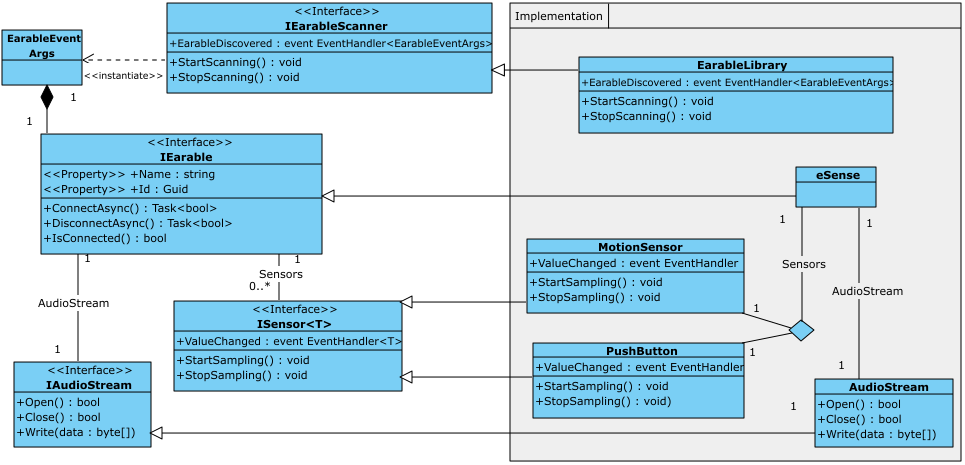
\includegraphics[scale=0.65]{uml_diagramme/EarableLibrary.png}

\subsection{IEarableScanner}
\sign{public interface IEarableScanner}
\begin{center}
	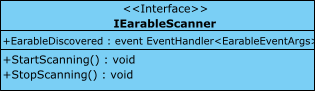
\includegraphics[scale=0.75]{EarableLibrary/IEarableScanner.png}
\end{center}
Stellt Interaktionsmöglichkeiten mit über Bluetooth verfügbaren Earable-Geräten bereit.
\paragraph{Events}
\begin{itemize}
	\i{event EventHandler<EarableEventArgs> EarableDiscovered} Erteilt jedes Mal eine Benachrichtigung, wenn bei aktiver Suche ein kompatibles Bluetooth-Gerät gefunden wurde.
\end{itemize}
\paragraph{Methoden}
\begin{itemize}
	\i{void StartScanning()} Startet die Suche nach Bluetooth-Geräten, falls nicht bereits aktiv.
	\i{void StopScanning()} Beendet die Suche nach Bluetooth-Geräten, falls aktiv.
\end{itemize}
\paragraph{Implementierung}
\begin{itemize}
	\i{EarableLibrary}
\end{itemize}

\subsection{EarableEventArgs}
\sign{public class EarableEventArgs : EventArgs}
\begin{center}
	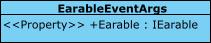
\includegraphics[scale=0.75]{EarableLibrary/EarableEventArgs.png}
\end{center}
Wird für \Gls{event}s verwendet, welche durch eine \code{IEarable} Instanz ausgelöst werden. Derart wird der Zugriff auf die auslösende Instanz ermöglicht.
\paragraph{Attribute}
\begin{itemize}
	\i{public IEarable Earable} Die das Event auslösende \code{IEarable} Instanz.
\end{itemize}

\subsection{IEarable}
\sign{public interface IEarable}
\begin{center}
	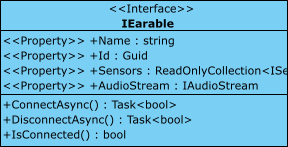
\includegraphics[scale=0.75]{EarableLibrary/IEarable.png}
\end{center}
Allgemeine Schnittstelle für Earable-Geräte.
\paragraph{Attribute}
\begin{itemize}
	\i{string Name} Ermöglicht zugriff auf den vergebenen Geräte-Namen.
	\i{Guid Id} Die Bluetooth-Adresse des Geräts.\glsnote{ro}
	\i{IAudioStream AudioStream} Zugehöriges AudioStream-Objekt.\glsnote{ro}
	\i{ReadOnlyCollection\footnote{System.Collections.ObjectModel.ReadOnlyCollection}<ISensor> sensors} Liste aller verfügbaren Sensoren.\glsnote{ro}
\end{itemize}
\paragraph{Methoden}
\begin{itemize}
	\i{Task\footnote{System.Threading.Tasks.Task}<bool> ConnectAsync()} Versucht asynchron eine Verbindung aufzubauen, sofern diese nicht bereits besteht.
	\i{Task<bool> DisconnectAsync()} Trennt die aktuelle Verbindung asynchron. Gibt \code{false} zurück, falls keine Verbindung besteht.
	\i{bool IsConnected()} Gibt einen Wahrheitswert zurück, der angibt, ob aktuell eine Verbindung besteht.
\end{itemize}
\paragraph{Mögliche Implementierungen}
\begin{itemize}
	\i{eSense}
\end{itemize}

\subsection{ISensor}
\sign{public interface ISensor}
\begin{center}
	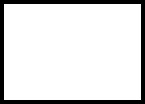
\includegraphics[scale=0.75]{EarableLibrary/ISensor.png}
\end{center}
Allgemeine Schnittstelle für Sensoren.
\paragraph{Events}
\begin{itemize}
	\i{event EventHandler ValueChanged} Erteilt Benachrichtigungen im Falle einer Messwertaktualisierung.
\end{itemize}
\paragraph{Methoden}
\begin{itemize}
	\i{void StartSampling()} Aktiviert das Auslesen von Messwerten.
	\i{void StopSampling()} Beendet das Auslesen von Messwerten.
\end{itemize}
\paragraph{Mögliche Implementierungen}
\begin{itemize}
	\i{MotionSensor} Repräsentiert die im Earable verbauten Bewegungssensoren (Gyroskop, Accelerometer)
	\i{PushButton} Repräsentiert den im Earable verbauten Zwei-Zustands-Knopf.
\end{itemize}

\subsection{IAudioStream}
\sign{public interface IAudioStream}
\begin{center}
	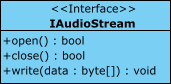
\includegraphics[scale=0.75]{EarableLibrary/IAudioStream.png}
\end{center}
Schnittstelle für einen Audio-Ausgabe-Stream.
\paragraph{Methoden}
\begin{itemize}
	\i{bool Open()} Öffnet den Stream.
	\i{bool Close()} Schließt den Stream.
	\i{void Write(byte[] data)} Hängt Audiodaten an den Buffer des AudioStreams an.
\end{itemize}
\paragraph{Implementierung}
\begin{itemize}
	\i{AudioStream}
\end{itemize}

\end{document}
